As described earlier, moving the arm's end effector to a desired position in space relative to the world frame is a forward kinematics problem. However, for a vehicle, moving to a position in space is primarily a velocity kinematics problem, because the velocity of the vehicle body has to be maintained over a period of time, which implies that the speeds for the wheels have to be coordinated to follow a specified path. \\

While this vehicle is technically a \ac{5DOF} vehicle, because the chassis can rotate about both its long and short axes with the joints attached to its legs, its basic pose can be described as an x and y coordinate pair with an orientation that the vehicle is facing $\theta$. Movement between an initial pose $[x_{i} \; y_{i} \; \theta_{i}]$ and final pose $[x_{f} \; y_{f} \; \theta_{f}]$ such as this can be thought of an initial turn, a straight movement, and then a final turn to get to the desired orientation. A top view example of this geometry can be seen in Figure~\ref{sample_return_rover:vel_kin:top_view}. Each set of concentric circles is an illustration of the path that a vehicle following an Ackerman model takes. The inner ring is the path for the inside wheels, the middle ring is the path of the lateral center of the chassis, and the outer ring is the path of the outer wheels.

\begin{figure}[H]
	\centering
	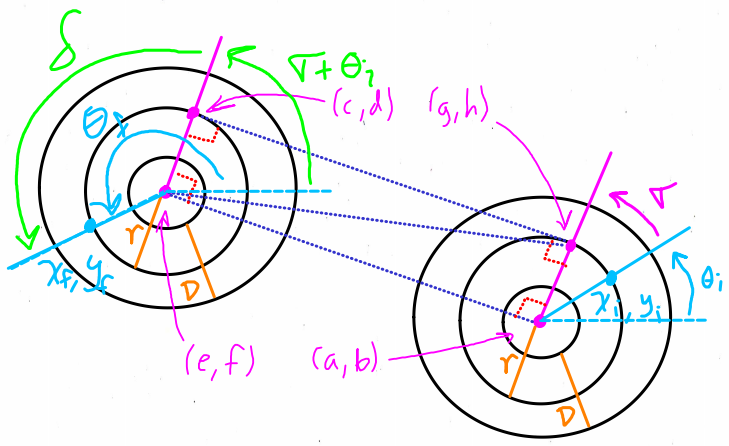
\includegraphics[width=\textwidth]{sections/robot-design/images/vel_kin_top_view.png}
	\caption{Overhead View of Example Vehicle Velocity Kinematics Problem}
	\label{sample_return_rover:vel_kin:top_view}
\end{figure}

\section{Calculate Displacements}
First, the distances traveled in each of these three movement segments need to be calculated. These are the arc of the first turn $\sigma$, the length of the linear movement between (g,h) and (c,d) $L$, and then the arc of the second turn $\delta$. To simplify the problem, the steering angle for the inner wheel is assumed to be the sharpest turn allowed, which means the distance between the \ac{ICC} and the later center of the vehicle is known. This allows for the values of \textit{a}, \textit{b}, \textit{e}, and \textit{f} to be calculated in terms of the initial and final positions of the vehicle, according to Equations~\ref{sample_return_rover:vel_kin:a} to~\ref{sample_return_rover:vel_kin:f}.

\begin{equation}\label{sample_return_rover:vel_kin:a}
	a = x_{i} - rc_{i}
\end{equation}

\begin{equation}\label{sample_return_rover:vel_kin:b}
	b = y_{i} - rs_{i}
\end{equation}

\begin{equation}\label{sample_return_rover:vel_kin:e}
	e = x_{f} - rc_{f}
\end{equation}

\begin{equation}\label{sample_return_rover:vel_kin:f}
	f = y_{f} - rs_{f}
\end{equation}

Where again:

\begin{equation}\label{sample_return_rover:vel_kin:csif}
	c_{i,f} = cos(\theta_{i,f}), \; s_{i,f} = sin(\theta_{i,f})
\end{equation}

Now consider the geometry of the triangle formed by points (e,f), (a,b), and (g,h), as seen in Figure~\ref{sample_return_rover:vel_kin:solving_g}. Solving for the position g would then allow to solve for the initial arc of the vehicle's movement $\sigma$, as seen in Equation~\ref{sample_return_rover:vel_kin:g_sigma}, and can be solved after finding the value for the angle $\beta$.

\begin{figure}[H]
	\centering
	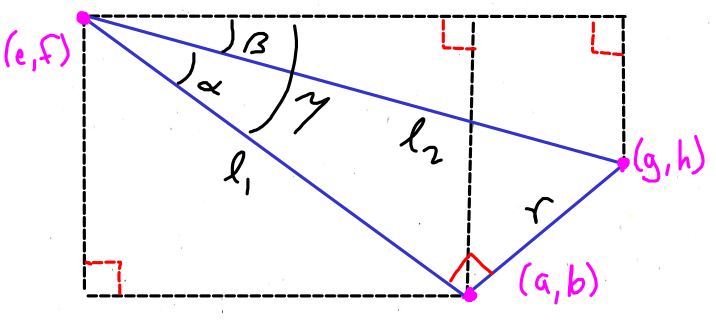
\includegraphics[width=0.8\textwidth]{sections/robot-design/images/vel_kin_solving_g.png}
	\caption{Triangle Formed by Velocity Kinematics Coordinates of Interest}
	\label{sample_return_rover:vel_kin:solving_g}
\end{figure}

\begin{equation}\label{sample_return_rover:vel_kin:g_sigma}
	\begin{split}
		g & = a + rc_{\sigma\theta_{i}} \\
		& = x_{i} - rc_{i} + rc_{\sigma\theta_{i}}
	\end{split}
\end{equation}

$\beta$ can be calculated according to Equation~\ref{sample_return_rover:vel_kin:beta}:

\begin{equation}\label{sample_return_rover:vel_kin:beta}
	\beta = \gamma - \alpha
\end{equation}

Therefore, the values of $\gamma$ and $\alpha$ must be solved for. Equation~\ref{sample_return_rover:vel_kin:gamma} describes how $\gamma$ can be easily calculated:

\begin{equation}\label{sample_return_rover:vel_kin:gamma}
	\gamma = atan2(f-b, \; a-e)
\end{equation}

Given Equations~\ref{sample_return_rover:vel_kin:a} to~\ref{sample_return_rover:vel_kin:f}, the distance $l_{1}$ is known according to Equation~\ref{sample_return_rover:vel_kin:l1}. This can be used to calculate $\alpha$, as seen in Equation~\ref{sample_return_rover:vel_kin:alpha}.

\begin{equation}\label{sample_return_rover:vel_kin:l1}
	l_{1} = \sqrt{(a-e)^2 + (f-b)^2}
\end{equation}

\begin{equation}\label{sample_return_rover:vel_kin:alpha}
	\alpha = -atan\left(\frac{r}{l_{1}}\right)
\end{equation}

Substituting Equations~\ref{sample_return_rover:vel_kin:gamma} and~\ref{sample_return_rover:vel_kin:alpha} into~\ref{sample_return_rover:vel_kin:beta} results in Equation~\ref{sample_return_rover:vel_kin:beta_expanded}.

\begin{equation}\label{sample_return_rover:vel_kin:beta_expanded}
	\beta = atan2(f-b, \; a-e) + atan\left(\frac{r}{l_{1}}\right)
\end{equation}

Because the values of $\alpha$ and $l_{1}$ are known, $l_{2}$ can be calculated as such:

\begin{equation}\label{sample_return_rover:vel_kin:l2}
	l_{2} = \sqrt{l_{1}^2 + r^2}
\end{equation}

Finally, g can be put into terms of $\beta$ geometrically and simplified using Equation~\ref{sample_return_rover:vel_kin:e}, according to Equation~\ref{sample_return_rover:vel_kin:g_beta}.

\begin{equation}\label{sample_return_rover:vel_kin:g_beta}
	\begin{split}
		g & = e + l_{2}c_{\beta} \\
		& = x_{f} - rc_{f} + l_{2}c_{\beta}
	\end{split}
\end{equation}

Combining Equations~\ref{sample_return_rover:vel_kin:g_sigma} and~\ref{sample_return_rover:vel_kin:g_beta} yields Equation~\ref{sample_return_rover:vel_kin:g_combined} and can be rearranged to solve for $\sigma$ according to ~\ref{sample_return_rover:vel_kin:sigma}. The relationship between $\delta$ and $\sigma$ is straightforward, as seen in Equation~\ref{sample_return_rover:vel_kin:g_combined}

\begin{equation}\label{sample_return_rover:vel_kin:g_combined}
	x_{i} - rc_{i} + rc_{\sigma\theta_{i}} = x_{f} - rc_{f} + l_{2}c_{\beta}
\end{equation}

\begin{equation}\label{sample_return_rover:vel_kin:sigma}
	\sigma = acos\left(\frac{x_{f} - x_{i} + l_{2}c_{\beta}}{r} + c_{i} - c_{f}\right) - \theta_{i}
\end{equation}

\begin{equation}\label{sample_return_rover:vel_kin:delta}
	\delta = \theta_{f} - \theta_{i} - \sigma
\end{equation}

Finally, $L$ has already implicitly been solved for, as the distance between (e,f) and (a,b) is the same as that of (c,d) and (g,h). Therefore:

\begin{equation}\label{sample_return_rover:vel_kin:L}
	L = l_{1}
\end{equation}

\section{Calculate Wheel Velocities and Estimated Elapsed Time}
Now that the values of $\sigma$, $L$, and $\delta$ are known, and while utilizing a simple assumption, all of the wheel velocities during the three movement segments, and the time each of those moves would ideally take, can be calculated. The arc length for the vehicle's outer wheels during the first turn, $S_{oft}$, can be calculated according to Equation~\ref{sample_return_rover:vel_kin:Soft}.

\begin{equation}\label{sample_return_rover:vel_kin:Soft}
	S_{oft} = R_{w}\Delta\omega_{oft}
\end{equation}

Where $R_{w}$ is the radius of the vehicle's wheels. The total rotation for the outside wheels $\Delta\omega_{oft}$ can also be calculated as the wheel's angular velocity over a period of time, according to Equation~\ref{sample_return_rover:vel_kin:delta_omegao}.

\begin{equation}\label{sample_return_rover:vel_kin:delta_omegao}
	\Delta\omega_{oft} = \dot{\omega_{oft}}\Delta t_{ft}
\end{equation}

The subscript for $\Delta t_{ft}$ does not include the 'o' because the elapsed time for the outside wheels is the same as the inside wheels over the course of the turn, which is a necessary conclusion to utilize later. \\

The aforementioned simple assumption is that the outside wheels during a turn will move at the peak velocity, which is a guaranteed safe assumption according to the Ackerman steering model, because the wheels must rotate slower to maintain a constant \ac{ICC}. Therefore:

\begin{equation}\label{sample_return_rover:vel_kin:omega_doto}
	\dot{\omega} = \dot{\omega}_{max}
\end{equation}

Rearranging the combination of Equations~\ref{sample_return_rover:vel_kin:Soft} to~\ref{sample_return_rover:vel_kin:omega_doto} to solve for the elapsed time yields Equation~\ref{sample_return_rover:vel_kin:delta_tft}.

\begin{equation}\label{sample_return_rover:vel_kin:delta_tft}
	\Delta t_{ft} = \frac{S_{oft}}{R_{w} \cdot \dot{\omega}_{max}}
\end{equation}

Equations~\ref{sample_return_rover:vel_kin:Sift} and~\ref{sample_return_rover:vel_kin:delta_omegai} are the same as the outside wheels except to reflect the inside wheels' movement. This time, $\Delta t_{ft}$ is not solved for, but is utilized to solve for the inside wheels' angular velocities, according to Equation~\ref{sample_return_rover:vel_kin:omega_doti}.

\begin{equation}\label{sample_return_rover:vel_kin:Sift}
	S_{ift} = R_{w}\Delta\omega_{ift}
\end{equation}

\begin{equation}\label{sample_return_rover:vel_kin:delta_omegai}
	\Delta\omega_{ift} = \dot{\omega_{ift}}\Delta t_{ft}
\end{equation}

\begin{equation}\label{sample_return_rover:vel_kin:omega_doti}
	\dot{\omega}_{ift} = \frac{S_{ift}}{R_{w} \cdot \Delta t_{ft}}
\end{equation}

For the second turn, the same exact process is utilized, except that the arc length of the distance traveled $S_{ift}$ is a function of $\delta$ instead of $\sigma$. \\

For the linear movement, because all the wheels must travel at the same speed to move straight, assume that all wheels can rotate at the peak wheel velocity. Similar to calculations for the turns, the distance traveled can be expressed as function of the angular displacement of the wheels, as well as the angular velocity of the wheels, which combined can solve for the elapsed time of the linear movement.

\begin{equation}\label{sample_return_rover:vel_kin:delta_omegam1}
	\Delta\omega_{m} = \frac{L}{R_{w}}
\end{equation}

\begin{equation}\label{sample_return_rover:vel_kin:delta_omegam2}
	\Delta\omega_{m} = \dot{\omega}_{m} \cdot \Delta t_{m}
\end{equation}

\begin{equation}\label{sample_return_rover:vel_kin:delta_tm}
	\Delta t_{m} = \frac{L}{R_{w} \cdot \Delta\omega_{m}}
\end{equation}
